%% -*- coding: utf-8 -*-
\documentclass[12pt,pagesize,paper=192mm:108mm,landscape]{scrbook} 
%1920x1080 1280x720
\areaset[current]{192mm}{108mm}
\usepackage{calc}
\usepackage[T2A]{fontenc}
\usepackage[utf8]{inputenc}
\usepackage[english,russian]{babel}
\usepackage{microtype}
\usepackage{misccorr}
\usepackage{cmap}
%\usepackage[unicode=true]{hyperref}
\usepackage{graphicx}
\usepackage{amssymb}
\usepackage{amsmath}
%\usepackage{srcltx}
\usepackage{textcomp}
\usepackage{xspace}
%научные символы и смайлики \smiley \frownie
\usepackage{wasysym}
\usepackage{ccicons}
\begin{document}
\begin{titlepage}
  \vspace*{-0.5em}
  \begin{center}    
    \hspace*{3em}
    \begin{minipage}[t]{1.5em}
      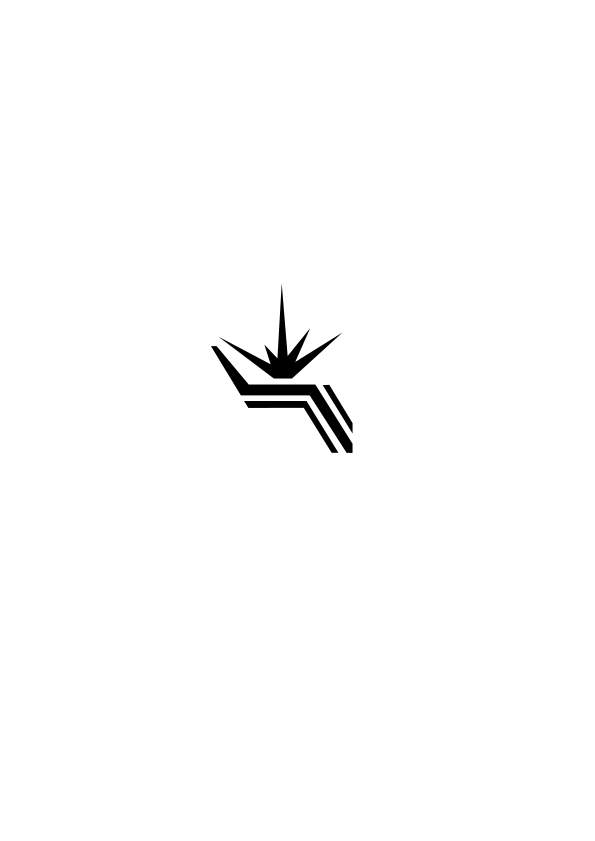
\includegraphics[width=\textwidth]{../BINP-logo}
    \end{minipage}\hfill
    \begin{minipage}{0.115\linewidth}
    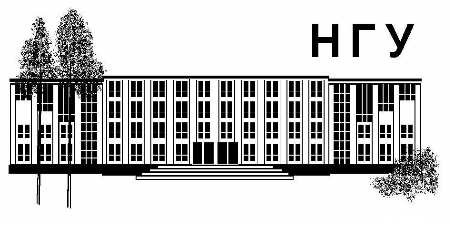
\includegraphics[width=\textwidth]{../NSU-logo}
    \end{minipage}
    \hfill
    \hspace*{4.5em}

    Кафедра теоретической физики физического факультета НГУ
    \medskip

    \Large
    Профессор Грабовский А.\,В.
    \smallskip

    \huge
    \textbf{Общая теория относительности}
    \smallskip

    \Large
    Семинар № 9
    \vfill

    \normalsize
    \begin{minipage}{0.83\linewidth}
      Вычисление квадрата тензора квадрупольного момента в поперечно
      бесследовой калибровке. Усреднение этой свертки по направлениям
      излучения гравитационной волны. Вычисление интенсивности
      излучения гравитационных волн двойной системой из звезд равной
      массы, вращающихся по круговой орбите. Вычисление скорости
      изменения периода обращения этой системы за счет излучения
      гравитационных волн. Оценка времени остывания белого карлика
      солнечной массы от $T\sim10^7$\,K.
    \end{minipage}
    \vfill

    \normalsize \ccbysa\hspace{0.5em}  Новосибирск 2022
  \end{center}
\end{titlepage}
\end{document}
